\documentclass{article}

\usepackage[left=2cm, right=2cm, top=2cm, bottom=2cm]{geometry}
\usepackage{fancyhdr}
\usepackage{float}
\usepackage{graphicx}
\graphicspath{{./images}}
\usepackage{hyperref}

\renewcommand{\figurename}{Ábra}

\pagestyle{fancy}
\lhead{Webes alkalmazások fejlesztése}
\rhead{2023/2024 tavaszi félév}
\cfoot{\thepage}

\begin{document}
	\section*{Beadandó feladat dokumentáció}
	\subsection*{Feladat}
	Készítsünk egy mozi üzemeltető rendszert, amelyben egy webes felületen keresztül a nézők tekinthetik meg a moziműsort, valamint rendelhetnek jegyeket.
	\begin{itemize}
		\item A főoldalon megjelenik a napi program, azaz mely filmeket mikor vetítik a moziban, valamint kiemelve az öt legfrissebb (legutoljára felvitt) film plakátja.
		\item A filmet kiválasztva megjelenik annak részletes leírása (rendező, főszereplők, hossz, szinopszis), plakátja, továbbá az összes előadás időpontja.
		\item Az időpontot kiválasztva lehetőség nyílik helyfoglalásra az adott előadásra. Ekkor a felhasználónak meg kell adnia a lefoglalandó ülések helyzetét (sor, illetve oszlop) egy, a mozitermet sematikusan ábrázoló grafikus felületen. Egyszerre legfeljebb 6 jegy foglalható, és természetesen csak a szabad helyek foglalhatóak (amelyek nem foglaltak, vagy eladottak). A felhasználónak ezen felül meg kell adnia teljes nevét, valamint telefonszámát, ezzel véglegesíti a foglalást.
	\end{itemize}
	\subsection*{Elemzés}
	\begin{itemize}
		\item A feladatot kettő komponens, egy adatbázis és egy webes felhasználói felület, mely utóbbi az Entity Framework segítségével az adatbázishoz kapcsolódva, ASP.NET Core-ban, MVC architekturával kerül megvalósításra.
		\item A feladat három weblapon fog megjelenni:
		\begin{enumerate}
			\item weblap a főoldal, melyen megjelenik a napi program, azaz mely filmeket mikor vetítik a moziban, valamint kiemelve az öt legfrissebb (legutoljára felvitt) film plakátja.
			\item weblap, mely az 1. weblapon való film választása után megjeleníti annak részletes leírását (rendező, főszereplők, hossz, szinopszis), plakátját, továbbá az összes aznapi előadás időpontját.
			\item weblap, melyen a 2. weblapon való időpont kiválasztása után lehetőség nyílik helyfoglalásra az adott előadásra. Ekkor a felhasználónak meg kell adnia a lefoglalandó ülések helyzetét (sor, illetve oszlop) egy, a mozitermet sematikusan ábrázoló grafikus felületen. Egyszerre legfeljebb 6 jegy foglalható, és természetesen csak a szabad helyek foglalhatóak (amelyek nem foglaltak, vagy eladottak). A felhasználónak ezen felül meg kell adnia teljes nevét, valamint telefonszámát, ezzel véglegesíti a foglalást.
		\end{enumerate}
	\end{itemize}
	\subsection*{Felhasználói esetek}
	\begin{figure}[H]
		\centering
		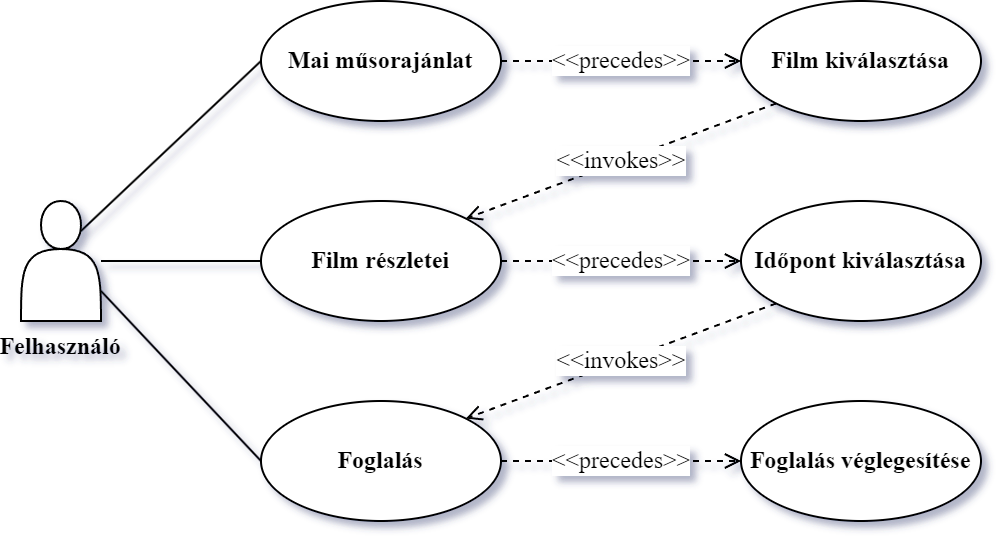
\includegraphics[width=0.75\textwidth]{usercase}
		\caption{Felhasználói esetek UML diagramja}
	\end{figure}
	\subsection*{Rendszer szerkezete}
	\begin{figure}[H]
		\centering
		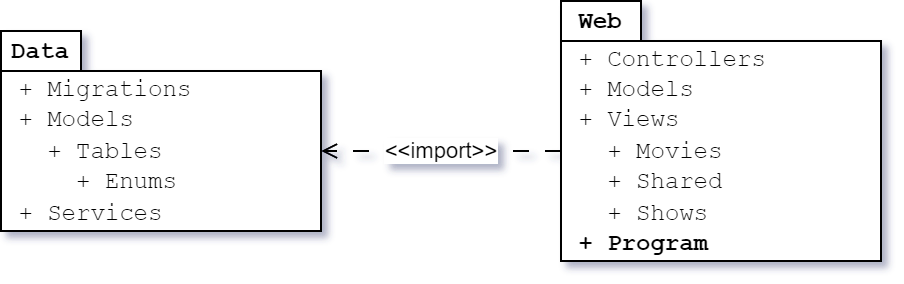
\includegraphics[width=0.75\textwidth]{component}
		\caption{Komponensek UML diagramja}
	\end{figure}
	\begin{itemize}
		\item A rendszer kettő projektből és azok névtereiből épül fel:
		\begin{enumerate}
			\item Az adatbázis modellt (\texttt{Models} és \texttt{Migrations} névterek) és annak szervízosztályát (\texttt{Services} névtér) tartalmazó \texttt{Cinema.Data} projekt
			\begin{enumerate}
				\item \texttt{Cinema.Data.Models} névtér az adatbázis sémájának és azok tábláinak definícióit tartalmazza, melynek tartalmát a \texttt{Cinema.Data.Migrations} névtérbe fordítja egy migráció esetén, mellyel futtatáskor áll fel az adatbázis
				\item \texttt{Cinema.Data.Services} névtér az adatbázis szervízosztályát tartalmazza, amely előre megírt lekérdezésekkel kommunikál a webes felület irányába
			\end{enumerate}
			\begin{figure}[H]
				\centering
				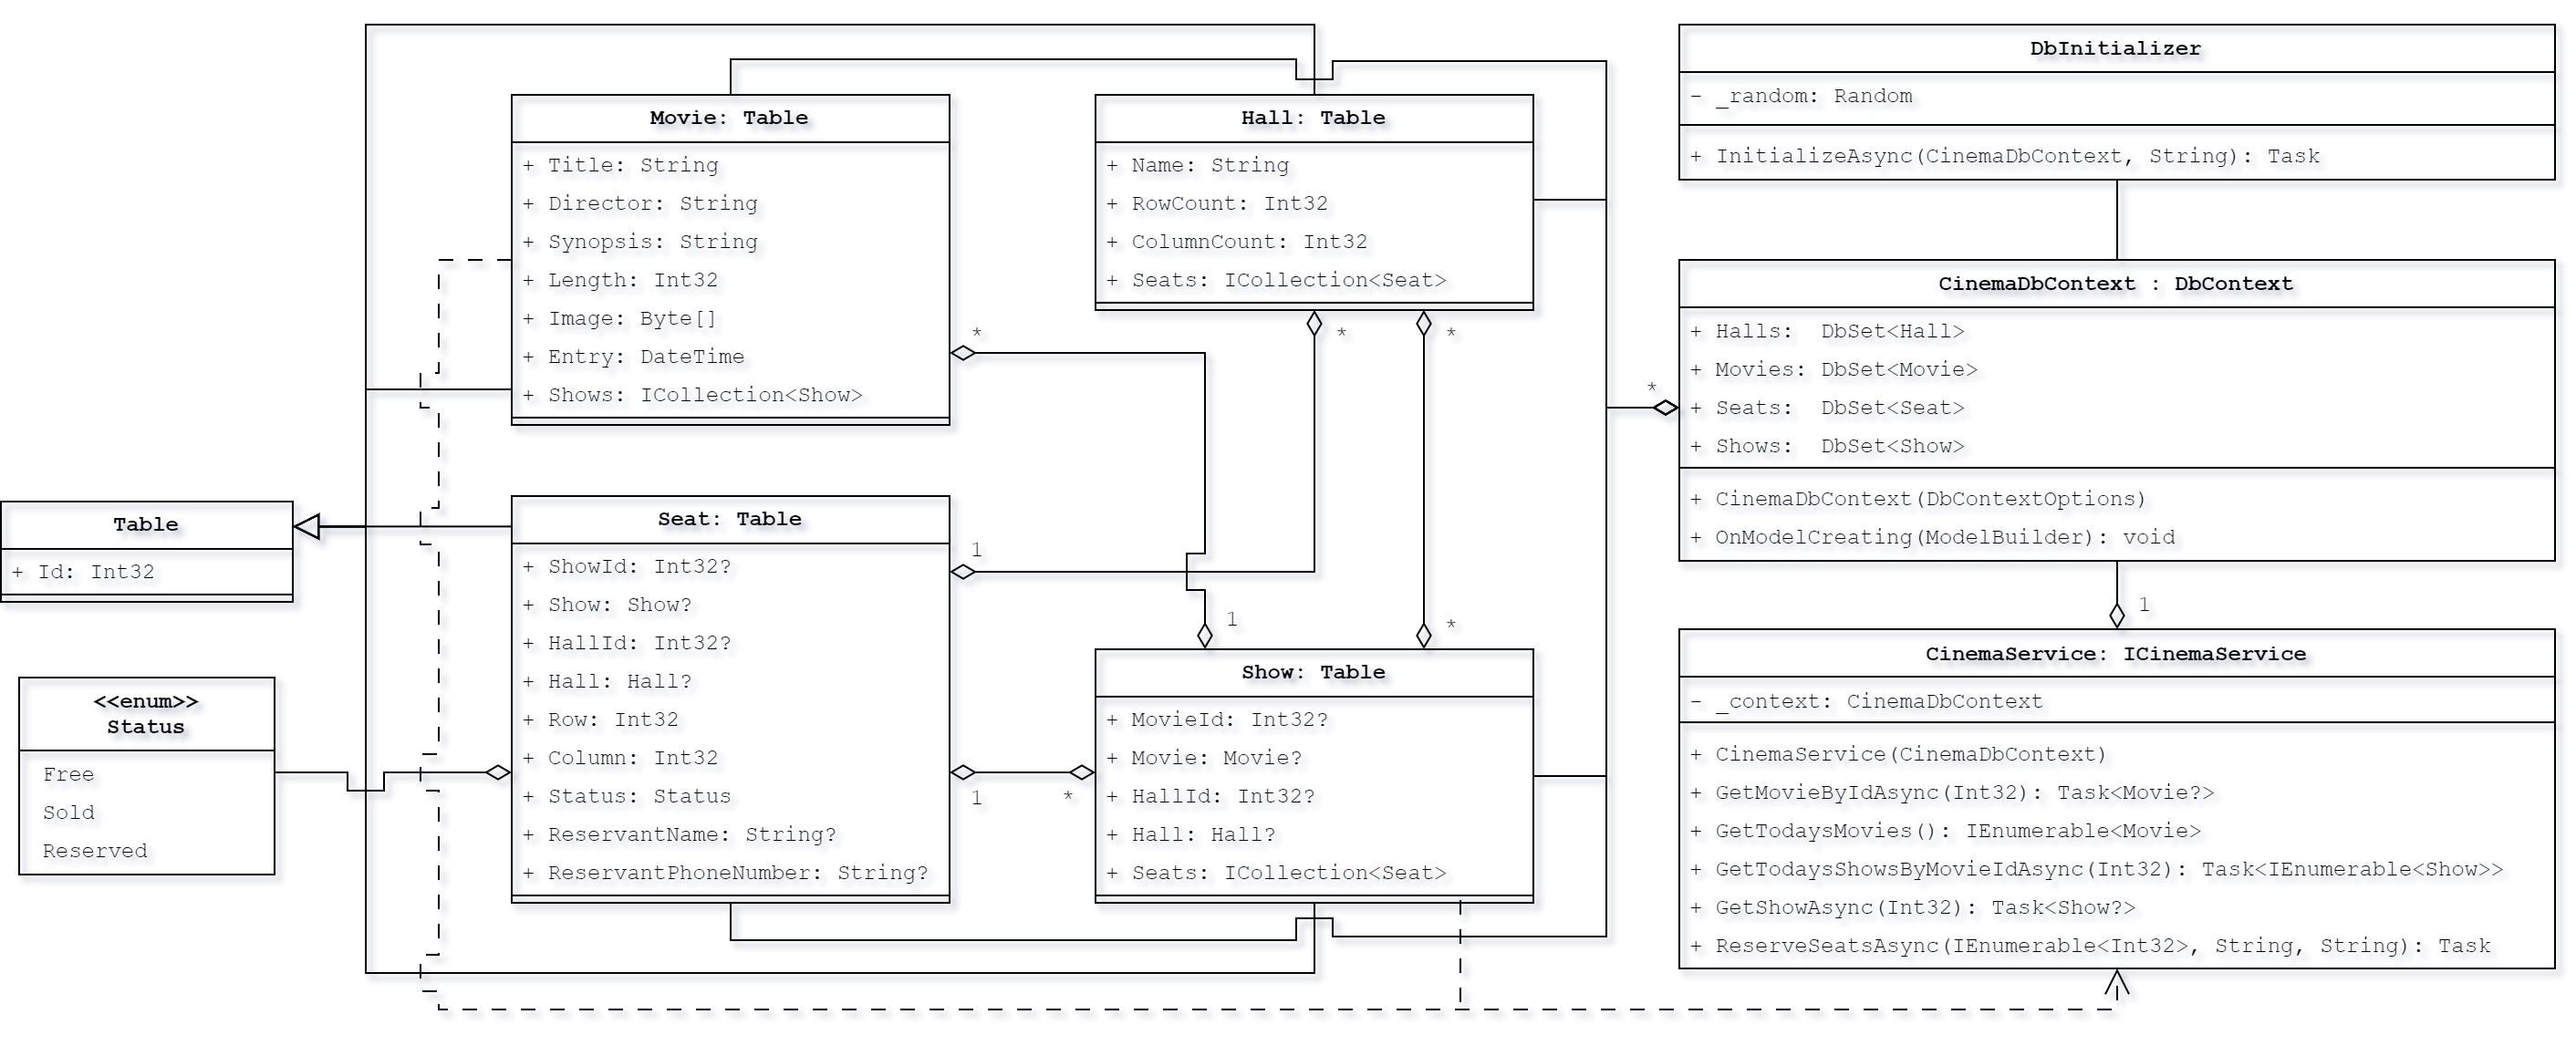
\includegraphics[width=1\textwidth]{data}
				\caption{A \texttt{Cinema.Data} projekt UML osztálydiagramja}
			\end{figure}\newpage
			\item A kontrollerosztályokat (\texttt{Controllers} névtér), az adatátviteli osztályokat (\texttt{Models} névtér) és a webes felhasználói felületet (\texttt{Views} névtér) tartalmazó \texttt{Cinema.Web} projekt
			\begin{enumerate}
				\item \texttt{Cinema.Web.Controllers} névtér az adatbázisból kapott szervízosztály előre megírt lekérdezéseinek az eredményét a \texttt{Cinema.Web.Models} névtérben definiált adatátviteli objektumokká alakítva továbbítja a webes felhasználói felület "dinamikus összeállítójának"
				\item \texttt{Cinema.Web.Views} névtér a webes felhasználói felület weblapjainak a "tervrajzait" tartalmazza \texttt{.cshtml} kiterjesztésben, amely a kapott adatoknak megfelelően szerveroldalon állítja össze a weblapot, majd küldi azt tovább a felhasználónak
			\end{enumerate}
			\begin{figure}[H]
				\centering
				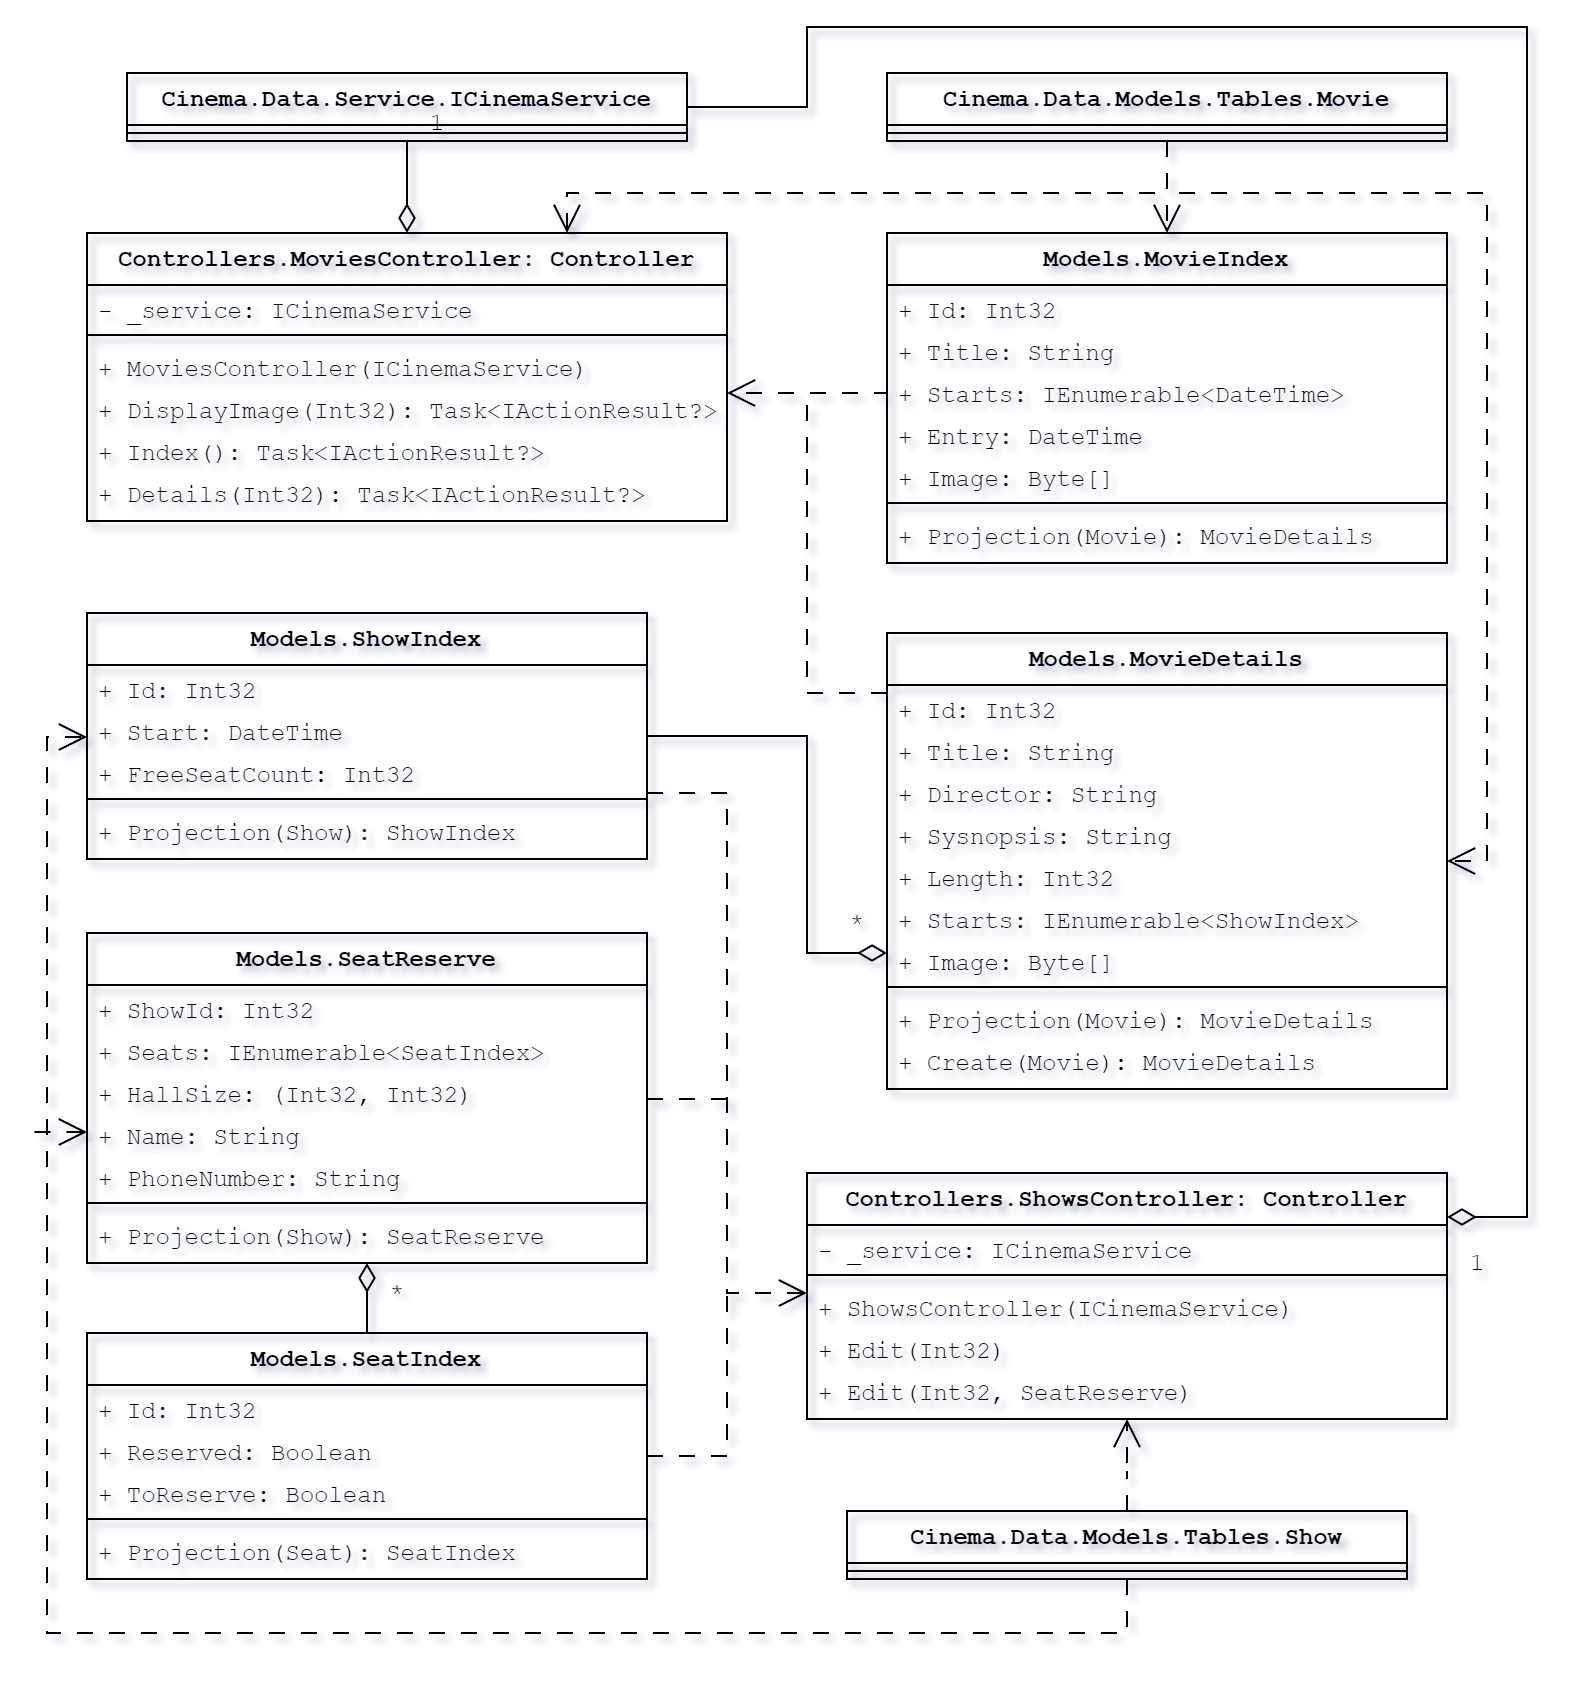
\includegraphics[width=\textwidth]{web}
				\caption{A \texttt{Cinema.Web} projekt UML osztálydiagramja}
			\end{figure}
		\end{enumerate}
	\end{itemize}
	\subsection*{Adatbázis felépítése}
	\begin{figure}[H]
		\centering
				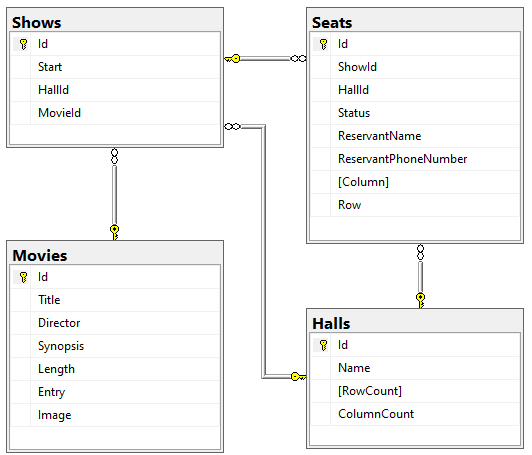
\includegraphics[width=\textwidth]{database}
		\caption{Az adatbázis sémájának diagramja}
	\end{figure}
\end{document}